\chapter{Instalaciòn Xilinx ISE y Xilinx EDK en Linux}\label{ApexA}



\section{Herramientas}

\begin{itemize}
 \item Linux Debian 6.0, Linux Fedora 17, CentOS 6.3
 \item Xilinx EDK 8.2.02 Build EDK\_Im\_Sp2.4
 \item Tarjeta de desarrollo NetFPGA
 \item Bibliotecas libusb y usb-driver
%  \item minicom
\end{itemize}


\section{Requerimeintos}

\section{Instalación del ISE y EDK}


Se deberá de  montar la imágen para acceder a los archivos. 
Para montar algún dispositivo o imágen se debe contar con privilegios de 
super-usuario:

  \begin{verbatim}	
   root@debian:~# mount -t iso9660 -o loop Xilinx_ISE_DS.iso /media/ 
  \end{verbatim}

La ruta de instalación será:

  \begin{verbatim}	
  #/mnt/setup 
  \end{verbatim}
  
\begin{figure}[ht]
  \begin{center}
 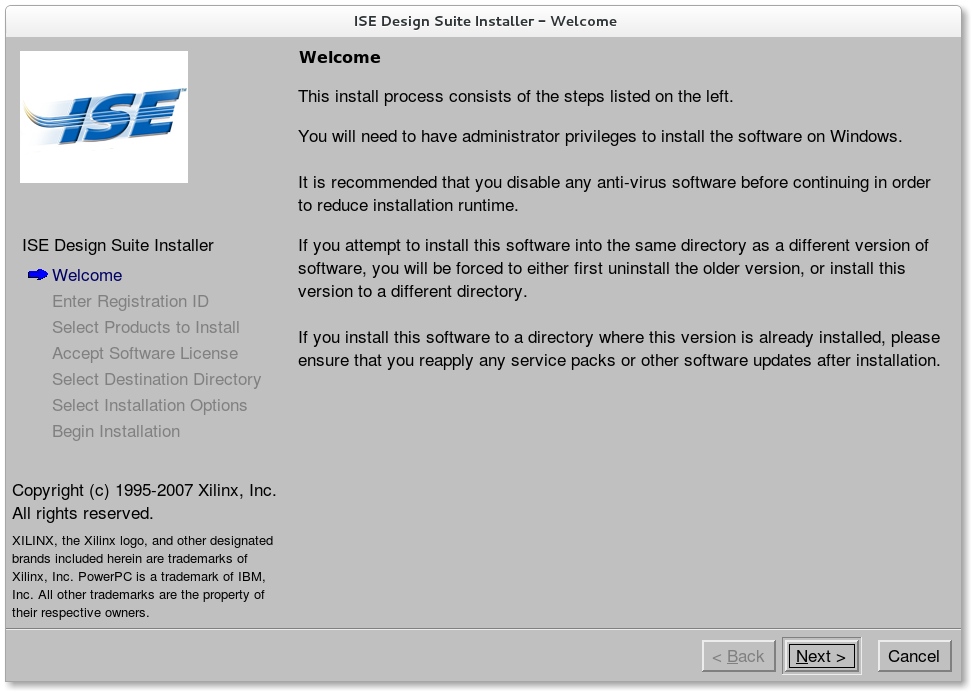
\includegraphics[scale=.40]{./figuras/Installer.png}
  \caption{Pantalla de instalaciòn ISE 8.2}
 \label{Pantalla instalaciòn ISE 8.2}
 % Installer.png: 971x691 pixel, 72dpi, 34.25x24.38 cm, bb=0 0 971 691
 \end{center}
\end{figure}

% Pass: 1472AKH27AD266UHKE980RNMB

En un sistema de escritorio personalizado la instalación creará un directorio
en su \emph{home} llamado Xilinx.

Seleccionamos solo los módulos que necesitamos:
\begin{itemize}
 \item Standalone Programming Tools
 \item ISE Design Tools
 \item Embedded Development Kit (EDK)
 \item ChipScope Pro
 \item PlanAhead Analysis Tool/PlanAhead Lite
\end{itemize}


\begin{figure}[ht]
  \begin{center}
 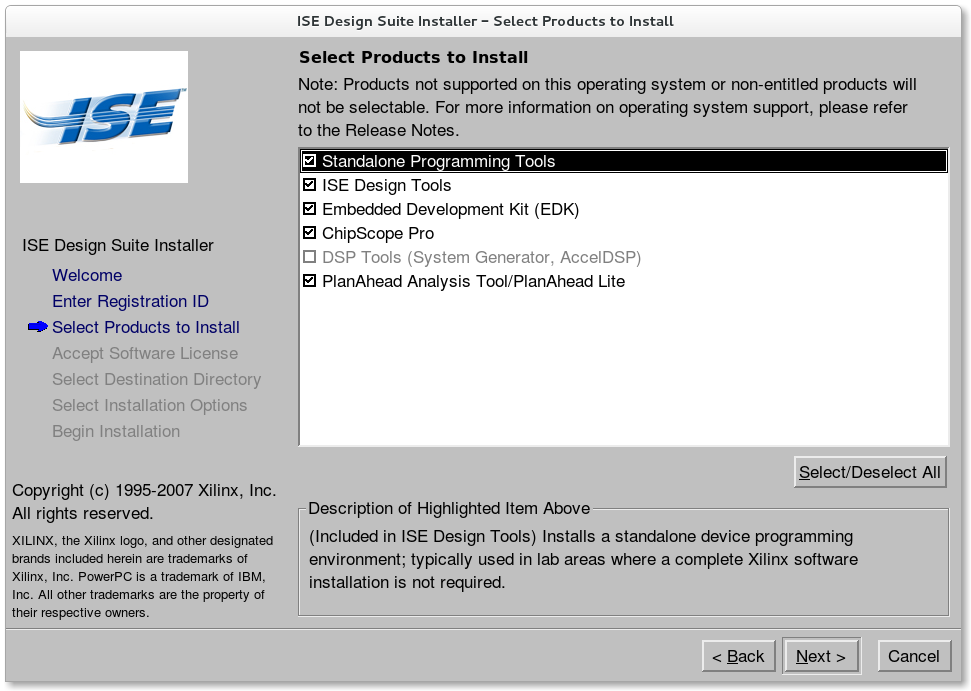
\includegraphics[scale=.40]{./figuras/Modules_install.png}
  \caption{Módulos a instalar}
 \label{Módulos a instalar ISE 8.2}
 % Installer.png: 971x691 pixel, 72dpi, 34.25x24.38 cm, bb=0 0 971 691
 \end{center}
\end{figure}

Se selecciona un directorio para a instalaciòn:

  \begin{verbatim}
  /opt/Xilinx/8.2 
  \end{verbatim}
  
  \begin{figure}[ht]
  \begin{center}
 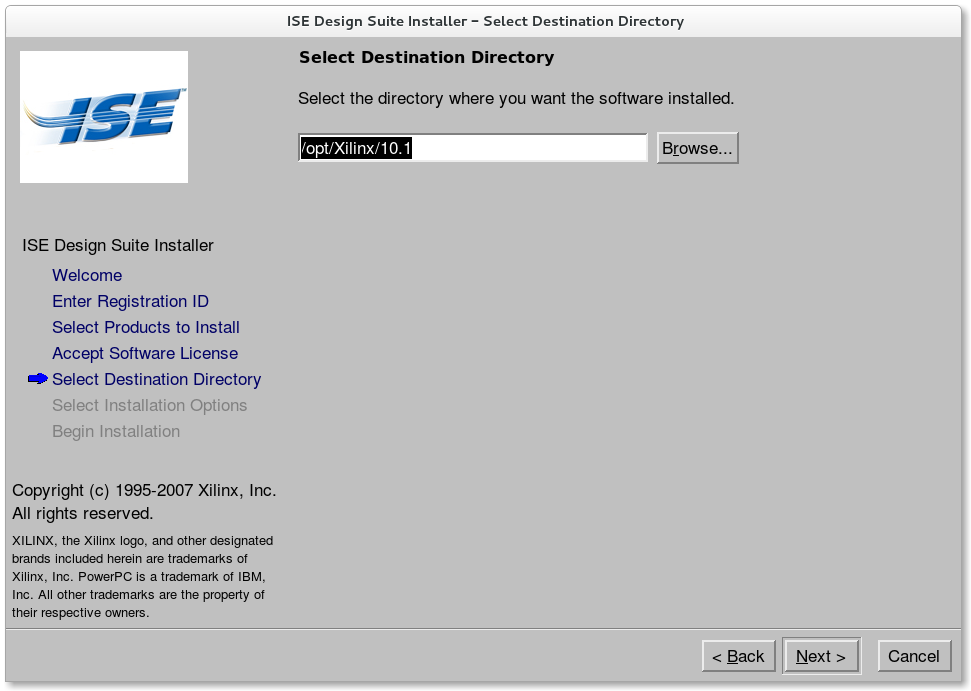
\includegraphics[scale=.40]{./figuras/Directory.png}
  \caption{Directorio de instalaciòn}
 \label{Directorio de instalaciòn ISE 8.2}
 % Installer.png: 971x691 pixel, 72dpi, 34.25x24.38 cm, bb=0 0 971 691
 \end{center}
\end{figure}

\section{Ejecución del ISE y EDK}


Para lanzar tanto ISE como el EDK, será necesario crear variables de ambiente
para la relación de sus aplicaciones, se han creado dos  \emph{scripts} que
facilitan la ejecución, \emph{ise.sh} permite la ejecución de ISE :

\lstinputlisting[caption=Archivo ise.sh,language=sh]{./code/ise.sh}

se agregan permisos de ejecución:

  \begin{verbatim}		
  root@debian:~$chmod +x ise.sh
  \end{verbatim}
 

\emph{edk.sh} permite la ejecución de EDK :

\lstinputlisting[caption=Archivo edk.sh,language=sh]{./code/edk.sh}

se agregan permisos de ejecución:

  \begin{verbatim}	
  Proyecto@debian:~$chmod +x edk.sh
  \end{verbatim}

 se edita el archivo \emph{.bashrc} quedando:
 \lstinputlisting[caption=Archivo .bashrc, language=sh,numbers=none,
]{./code/bashrc}
  
 
  
  se procede a ejecutar ISE :
  
    \begin{verbatim}		
  Proyecto@debian:~$ise
  \end{verbatim}
  
    \begin{figure}[ht]
  \begin{center}
 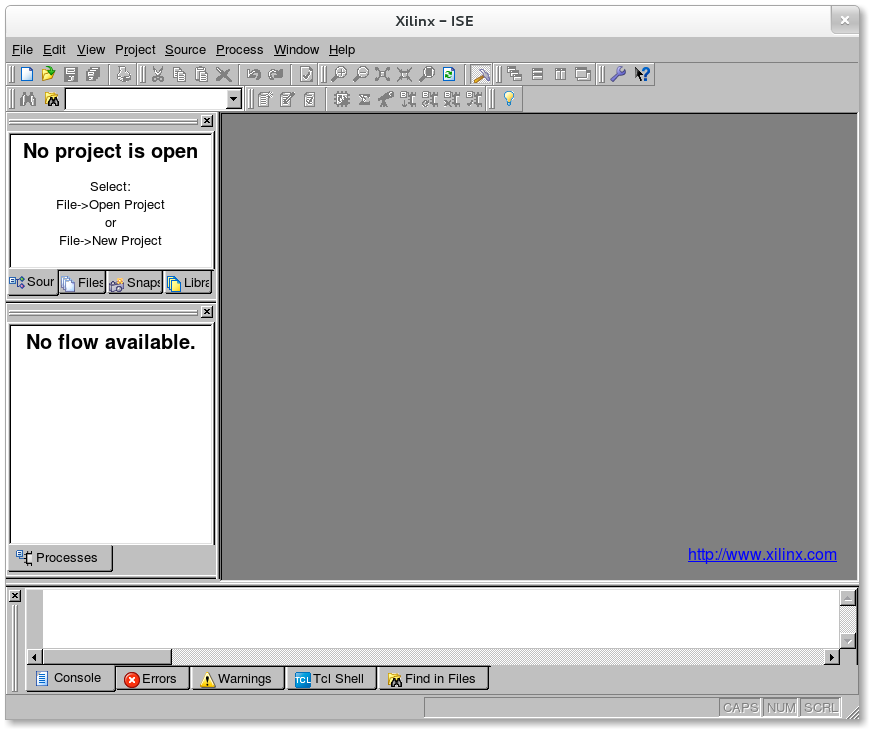
\includegraphics[scale=.40]{./figuras/ise.png}
  \caption{Ejecución de ISE 8.2}
 \label{Ejecución de ISE 8.2}
 % Installer.png: 971x691 pixel, 72dpi, 34.25x24.38 cm, bb=0 0 971 691
 \end{center}
\end{figure}

 por ultimo se ejecuta EDK :
 
     \begin{verbatim}		
  Proyecto@debian:~$edk
  \end{verbatim}
  
    \begin{figure}[ht]
  \begin{center}
 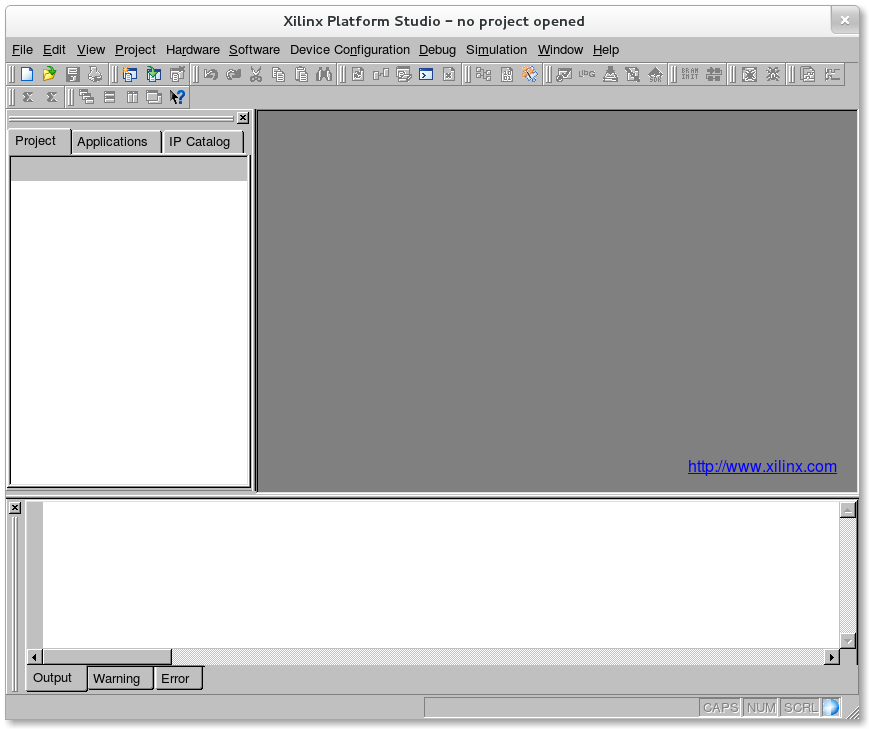
\includegraphics[scale=.40]{./figuras/edk.png}
  \caption{Ejecución de EDK 8.2}
 \label{Ejecución de EDK 8.2}
 % Installer.png: 971x691 pixel, 72dpi, 34.25x24.38 cm, bb=0 0 971 691
 \end{center}
\end{figure}
  
  


